% 	HTML5 Robot User Interface Project Report: Summary
% 	An ASLab Project,
% 	Developed by Daniel Peiró
% 	ETSII, UPM 2014-2015
\chapter{Resumen Ejecutivo\\(Executive Summary in Spanish)}

El objetivo de este proyecto es el desarrollo de \textit{software} que proporcione una interfaz gŕafica de usuario (en adelante 
\textit{GUI}) con una variedad de herramientas diseñadas para recoger entradas (\textit{inputs}) para el control de robots, asi 
como la presentación de las salidas (\textit{outputs}) de los mismos. Se desea que la aplicación (el programa) cumpla con los 
siguientes requisitos:
\begin{itemize}
	\item \textbf{Universalidad}: La GUI debe ser fácilmente adaptable al uso de un amplio abanico de robots, con diferentes 
	capacidades y características.
	\item \textbf{Accesibilidad}: Este requisito se divide en dos partes:
	\begin{itemize}
		\item La GUI debe ser fácilmente utilizable desde un amplio abanico de dispositivos, incluyendo como mínimo, 
		ordenadores de sobremesa (\textit{desktop}) y portátiles (\textit{laptop}), dispositivos móviles como teléfonos 
		inteligentes (\textit{smartphones}) y tabletas (\textit{tablets}), todos ejecutando distintos sistemas operativos, con 
		respecto a los cuales la aplicación debería ser agnóstica (debería ejecutarse indistintamente en cualquier SO).		
		\item La aplicación que proporcione la GUI debe además exponer una API (\textit{Application Programming Interface} o 
		Interfaz de Programación de la Aplicación) que permita a desarrolladores externos usar las entradas y salidas de la GUI 
		para cualquier robot o aplicación, consiguiendo asi realizar el primer requisito. Esta interfaz debe ser tan simple 
		como sea posible, y debe cumplir con todos los demás requisitos, donde sea aplicable (por tanto debe ser portable, 
		distribuida, en tiempo real y de código abierto (\textit{open source})).
	\end{itemize}
	\item \textbf{Personalizable (\textit{Customizable})}: Parcialmente debido al primer requisito, la GUI debe tener una 
	variedad de entradas y salidas que deben ser utilizables de manera independiente, de tal forma que múltiples 
	configuraciones puedan prepararse y ser usadas para diferentes robots, asi como para diferentes aplicaciones del mismo 
	robot. A ser posible, el usuario debería poder crear entradas y salidas personalizadas cuando las herramientas propuestas 
	sean insuficientes para la aplicación particular. Este proceso debería ser sencillo y transparente para el usuario, a ser 
	posible.
	\item \textbf{Distribuida}: Parcialmente debido al requisito de accesibilidad, la aplicación debe ser distribuida en red, de 
	manera que la GUI no esté físicamente atada a una máquina en particular, o tenga que ser ejecutada de manera local para 
	aportar la funcionalidad requerida.
	\item \textbf{Tiempo Real}: Las entradas registradas por la GUI deben ser capaces de controlar al robot en tiempo real. 
	Asímismo, las salidas del robot deben ser presentadas al usuario en tiempo real. No se establecen tiempos límite 
	(\textit{deadlines}) severos, dado que la aplicación es distribuida y por tanto estos tiempos serían difíciles de estimar sin 
	una investigación exhaustiva y control sobre el entorno de ejecución de la aplicación, lo cual negaría el requisito de 
	accesibilidad. Sin embargo, el tiempo de respuesta del sistema deberá minimizarse dentro de las posibilidades del estado del 
	arte de las tecnologías empleadas.
	\item \textbf{Portabilidad}: La aplicación que proporcione la GUI debe ser ejecutable en un amplio abanico de sistemas, con 
	respecto a estas variables:
		\begin{itemize}
			\item Prestaciones \textit{Hardware}: La aplicación debe ser ejecutable en ordenadores portables de bajo coste y 
			bajas prestaciones con el fin de ser montable sobre robots móviles si así se requiere.
			\item Sistemas Operativos: La aplicación debe ser multi plataforma, es decir, debe ser ejecutable en una variedad de 
			sistemas operativos. Estos SOs deben incluir, como mínimo: una distribución de uso general de Linux, Microsoft 
			Windows y Apple OS X. Solo las últimas versiones de cada uno deben ser soportadas. Se requiere soporte como mínimo 
			las siguientes arquitecturas: 32/64-bit x86.\\
		\end{itemize}
	\item \textbf{Código Abierto (\textit{Open Source})}: Todo el \textit{software}, bibliotecas (\textit{libraries}) y 
	\textit{frameworks} empleados en el desarrollo y uso de la aplicación deben ser de código abierto. Esto, a grandes rasgos, 
	supone que el \textit{software} sea libre para el uso, estudio y modificación del mismo para cualquier propósito. Las 
	implicaciones del código abierto se estudian en la memoria del proyecto como valoración de los impactos y aspectos de 
	responsabilidad legal, ética y profesional del trabajo. Las herramientas usadas para el desarrollo (Entornos Integrados de 
	Desarrollo \textit{IDEs}, SOs, \textit{hardware} etc.) no tienen porque ser de código abierto, pero se preferirán 
	herramientas que lo sean en caso de ser alternativas viables.\\
\end{itemize}
En esencia, la aplicación debe establecer un nexo entre las dos entidades principales del control de robots:
\begin{itemize}
	\item \textbf{El Usuario}: Requiere una interfaz para introducir comandos que el robot debe seguir. Asímismo, requiere una 
	vista de las datos de salida del robot, si están disponibles.
	\item \textbf{El Robot}: Necesita recibir comandos en un protocolo particular que entiende, para poder funcionar. Además, 
	opcionalmente, puede exponer datos de salida para que el usuario los vea o sean registrados.
\end{itemize}
En el siguiente diagrama UML (\textit{Unified Modeling Language}) simplificado,se muestran los tres componentes: el usuario, la 
aplicación y el robot. El objetivo del proyecto es el desarrollo del componente central, la aplicación, junto con las interfaces 
que expone tanto al usuario como a robot, o con mayor precisión al controlador del robot, que traducirá la interfaz de la 
aplicación a la interfaz que entiende el robot.
\begin{figure}[H]
\centering
\captionsetup{justification=centering}
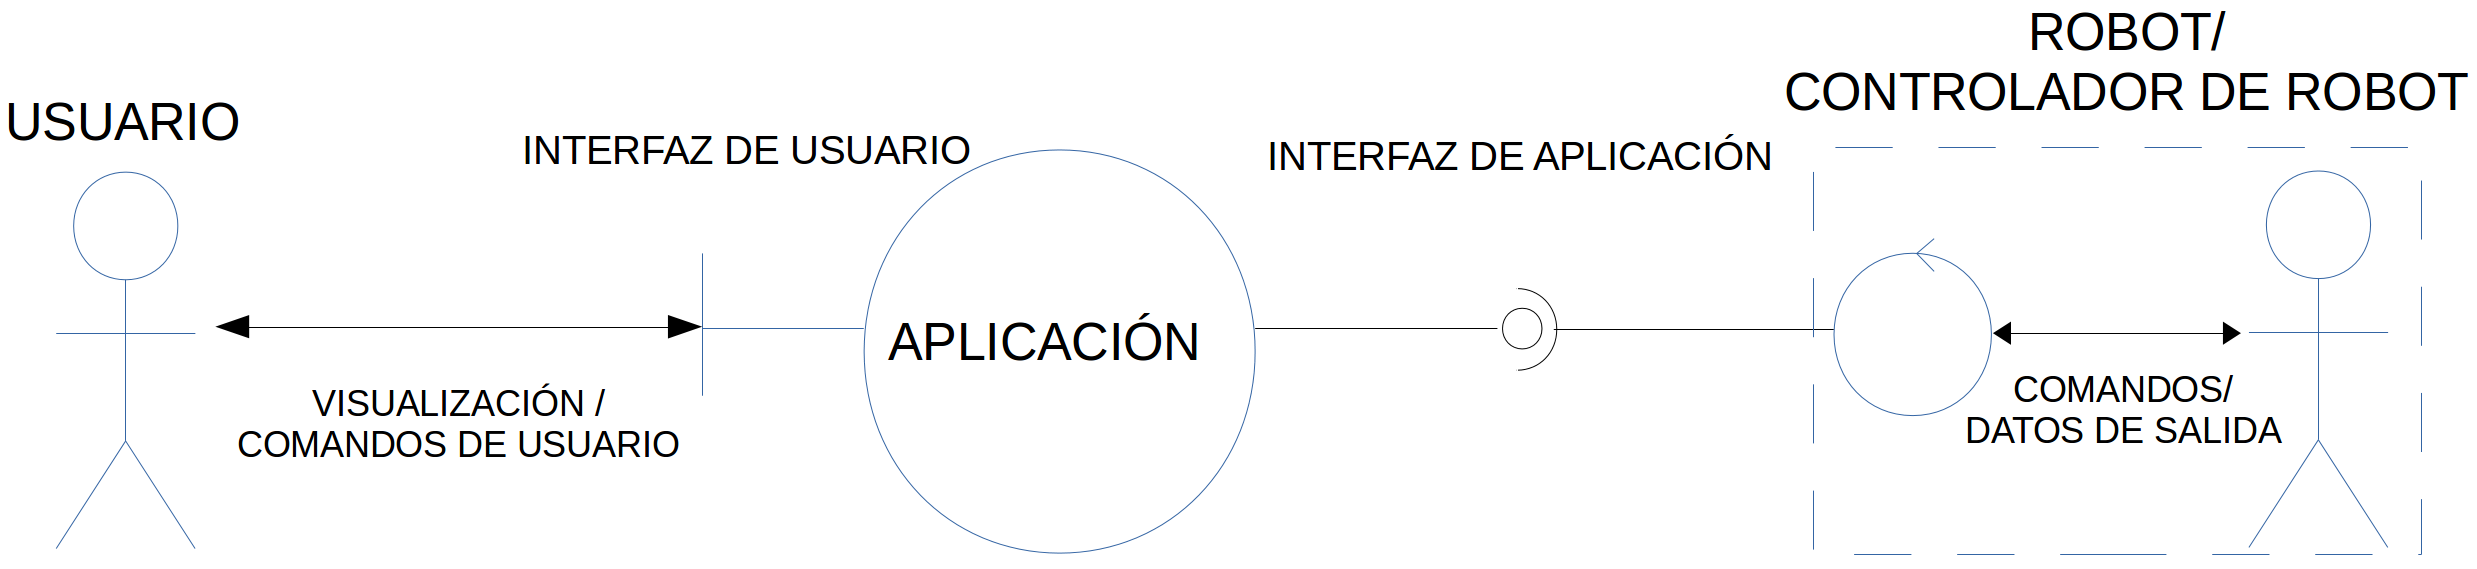
\includegraphics[width=\linewidth]{resumenuml}
\caption{Diagrama UML simplificado del objetivo del proyecto}
\end{figure}

Siguiendo un esquema de desarrollo en cascada iterativo (elaboración de requisitos, diseño, implementación y verificación, 
iterados para cada módulo de la aplicación, y finalmente mantenimiento), se planificó el proyecto. A continuación se procedió al 
estudio del estado del arte de las tecnologías que cumplen con estos requisitos y el diagrama de objetivos. Se diseñó una 
arquitectura del sistema que cumplía con los objetivos y se desarrolló la aplicación. Por último se probó el funcionamiento de la 
aplicación y se escribió la memoria del proyecto, en la que se describe en detalle el estado del arte de las tecnologías 
empleadas (capítulo 3), la arquitectura del sistema (capítulo 4), el desarrollo futuro (capítulo 5) y la planificación del 
proyecto (capítulo 6). Se incluye además como anexo el manual de usuario de la aplicación.\\

Los puntos básicos de la solución propuesta son los siguientes:
\begin{itemize}
	\item \textbf{GUI Modular en HTML5}: La GUI es una página web estrictamente en HTML5 (la última versión del estándar del 
	lenguaje empleado para diseñar páginas web). Esto propone una solución al requisito de accesibilidad, dado que las páginas 
	HTML5 son accesibles desde cualquier dispositivo capaz de abrir una página web. Esto incluye ordenadores, teléfonos 
	inteligentes y tabletas, así como una variedad de micro ordenadores. La modularidad proporciona una solución al requisito de 
	personalización, dado que cada módulo puede ejecutarse independientemente de otros, y por tanto cualquier permutación de 
	módules es posible.
	\item \textbf{Servidor Node.js}: La aplicación es un servidor web Node.js (una plataforma para ejecutar programas en el 
	lenguaje JavaScript como si fueran cualquier otro programa, en lugar de en el navegador. Está basado en el motor de 
	JavaScript de Google Chrome, es muy ligero y asíncrono). Dado que Node.js es multi plataforma, esto también aporta una 
	solución al requisito de portabilidad.
	\item \textbf{Arquitectura Cliente-Servidor}: Proporciona una solución al requisito  de ser una aplicación distribuida. El 
	clientes es la página web HTML5. El servidor es la aplicación que maneja las entradas y salidas del cliente. Pueden ser 
	ejecutados en máquinas distintas y se comunican vía Internet o en red local mediante varios protocolos.
	\item \textbf{Comunicación basada en \textit{WebSockets}}: Este protocolo de comunicación permite al cliente y servidor 
	comunicarse en tiempo real sobre una red de manera eficiente pasando mensajes entre ellos con paquetes de datos asociados, de 
	manera similar a los programas que se comunican entre sí mediante un \textit{socket} UNIX. Esto da respuesta al requisito de 
	tiempo real.
	\item \textbf{Arquitectura MVC (Modelo-Vista-Controlador)}: Propone una solución a los requerimientos de universalidad y 
	accesibilidad (segundo apartado), mediante el diseño de la aplicación. Se diseña de manera que la GUI (la Vista) está 
	desacoplada del estado de la aplicación (el Modelo), permitiendo así que desarrolladores externos accedan sencillamente al 
	Modelo, usando Controladores. Esto se llama doble-desacoplamiento (\textit{double-decoupling}) en el proyecto.
	\item \textbf{Entradas y salidas personalizables}: Como resultado de la prestación previa, el usuario puede crear nuevas 
	entradas y salidas dinámicamente, que son accesibles a la interfaz de la aplicación de manera instantánea y transparente. 
	Esto da respuesta al requisito de personalización.
	\item \textbf{Código abierto}: Todas las tecnologías empleados son de código abierto.
\end{itemize}
Los resultados del proyecto se detallan en el capítulo 7 de la memoria.\\

Como demostración del funcionamiento de la aplicación, se realizó la integración de la misma con tres robots distintos:
\begin{itemize}
	\item \textbf{Khepera III Virtual, en simulador V-REP}. Comunicado en Red.
	\item \textbf{Khepera III (Robot diferencial)}. Comunicado en Red inalámbrica.
	\item \textbf{Crazyflie 2.0. (Mini-Cuadrirotor)}. Comunicación por Radio.
	\item Parrot Rolling Spider (Mini-Cuadrirotor con estabilización de altura por ultra-sonidos). Comunicación por bluetooth. 
	(Nota: no documentado por ser muy parecido al anterior cuadrirotor).
\end{itemize}

Siendo las tres integraciones un éxito, ya que con controladores relativamente simples (el cuadrirotor requiere apenas 50 líneas 
de código para ser controlado totalmente en vuelo usando un mando con dos \textit{joysticks}) y en lenguajes de programación 
diferentes (la aplicación tiene interfaz con prácticamente cualquier lenguaje de programación moderno), se consiguió controlar y 
leer los datos en todos los casos en tiempo real, sin retrasos incluso usando redes móviles para la conexión vía internet.\\

Como demostración de la portabilidad de la aplicación, se integró en un micro ordenador de bajas prestaciones (4 núcleos a 900 
Mhz y 1 GB de RAM) y bajo coste (33 Euros), el Raspberry Pi 2. Esto permite, mediante una batería externa (5 V, 1.5 A), montar el 
micro ordenador (85x56x17 mm) en cualquier robot móvil, permitiendo su control vía internet desde cualquier dispositivo que pueda 
abrir un navegador, sin necesidad de ningún hardware intermedio (salvo, lógicamente la interfaz entre el micro ordenador y el 
robot, que comúnmente será en red TCP/IP, bluetooth, radio, serial, etc.).\\

La aplicación tiene las siguientes herramientas para uso con cualquier robot, otorgando una gran versatilidad:
\begin{itemize}
	\item \textbf{Módulos de entrada}: Utilizados para dar órdenes o de manera mas general, aportar datos a la aplicación y en 
	consecuencia al robot.
		\begin{itemize}
			\item Módulo de \textit{Joystick}: Joystick virtual, manipulable con el cursor o con el tacto (si el dispositivo es 
			táctil).
			\item Módulo \textit{Gamepad}: Permite conectar cualquier mando externo al dispositivo de control, y usarlo como 
			controlador del robot.
			\item Módulo de orientación del dispositivo: Permite usar los datos de orientación y movimiento del dispositivo como 
			controles para el robot (si el dispositivo tiene accelerómetros o equipos similares).
			\item Módulo de comandos por voz: Permite dar órdenes por voz al robot, mediante reconocimiento de lenguajes en línea 
			(requiere conexión a internet, disponible en varios idiomas, solo disponible en algunos navegadores).
			\item Módulo de entradas personalizadas: Permite al usuario crear entradas personalizadas (valores numéricos, 
			deslizadores, casillas booleanas o texto) dinámicamente y al instante, para suplir cualquier otro tipo de entrada no 
			contemplado.
		\end{itemize}
	\item \textbf{Módulos de salida}: Utilizados para presentar datos del modelo de la aplicación, normalmente datos del robot.
		\begin{itemize}
			\item Módulo de Monitorización de datos: Presenta la posición, orientación, velocidad y velocidad angular del robot, 
			además de un mapa de localización. El mapa puede ser generado dinámicamente, (útil para localización y mapeo 
			simultáneo, SLAM), puede ser estático en forma de imagen subida por el usuario o incluso pueden dibujarse obstáculos 
			dinámicamente con el cursor o tacto, para que sean reconocidos en tiempo real por el controlador del robot (mediante 
			una matriz binaria).
			\item Módulo de Vídeo en directo: Permite ver en directo una alimentación de vídeo proviniente de cualquier cámara 
			conectada al servidor. Útil para control remoto y FPV (vista en primera persona).
			\item Módulo de Audio en directo: Permite escuchar en directo (tiene un retraso de 2 segundos apróx.) una 
			alimentación de audio de cualquier fuente conectada al servidor.
			\item Módulo de Geolocalización: Presenta un mapa dinámico (usando Google Maps) de la geolocalización del robot, 
			siempre que se proporcionen los datos desde el robot a la aplicación.
			\item Módulo de salidas personalizadas: Permite al usuario visualizar cualquier dato de salida del robot que se 
			introduzca en la aplicación, que no haya sido contemplado por otro módulo.
		\end{itemize}
	\item \textbf{Módulos de Utilidad}: Disponibles para la comodidad del usuario.
		\begin{itemize}
			\item Módulo de ejecución de scripts: Permite al usuario ejecutar programas en el servidor de manera remota, siempre 
			que se hayan añadido a una localización concreta en el servidor (por seguridad).
			\item Módulo de administración de perfiles: Permite guardar y recuperar cualquier combinación de módulos con todos 
			sus datos, para poder configurar la interfaz de manera permanente para cada caso de uso. Útil particularmente para el 
			uso de gran cantidad de entradas personalizadas.
		\end{itemize}
\end{itemize}
El proyecto se realizó entre Agosto de 2014 y Agosto de 2015. Inicialmente debía entregarse en Marzo de 2015, pero debido a que 
el estudiante fue contratado como becario en Octubre de 2014, el trabajo del proyecto tuvo que relegarse al tiempo libre y fines 
de semana. La memoria está escrita en inglés porque al tratarse de un proyecto software, en el que la mayoría de los términos, 
lenguajes de programación, código escrito, comentarios de código, documentación de todos los sistemas empleados, fuentes de 
información etc. están en dicho idioma, se consideró más práctico el uso del mismo para documentar el proyecto.